\documentclass[tikz,border=8pt]{standalone}
\usepackage[utf8]{inputenc}
\usetikzlibrary{arrows.meta,fit,backgrounds,shadows}

% module names: smaller monospace so the longest ones fit in a block
\newcommand{\modname}[1]{{\scriptsize\ttfamily #1}}

\begin{document}
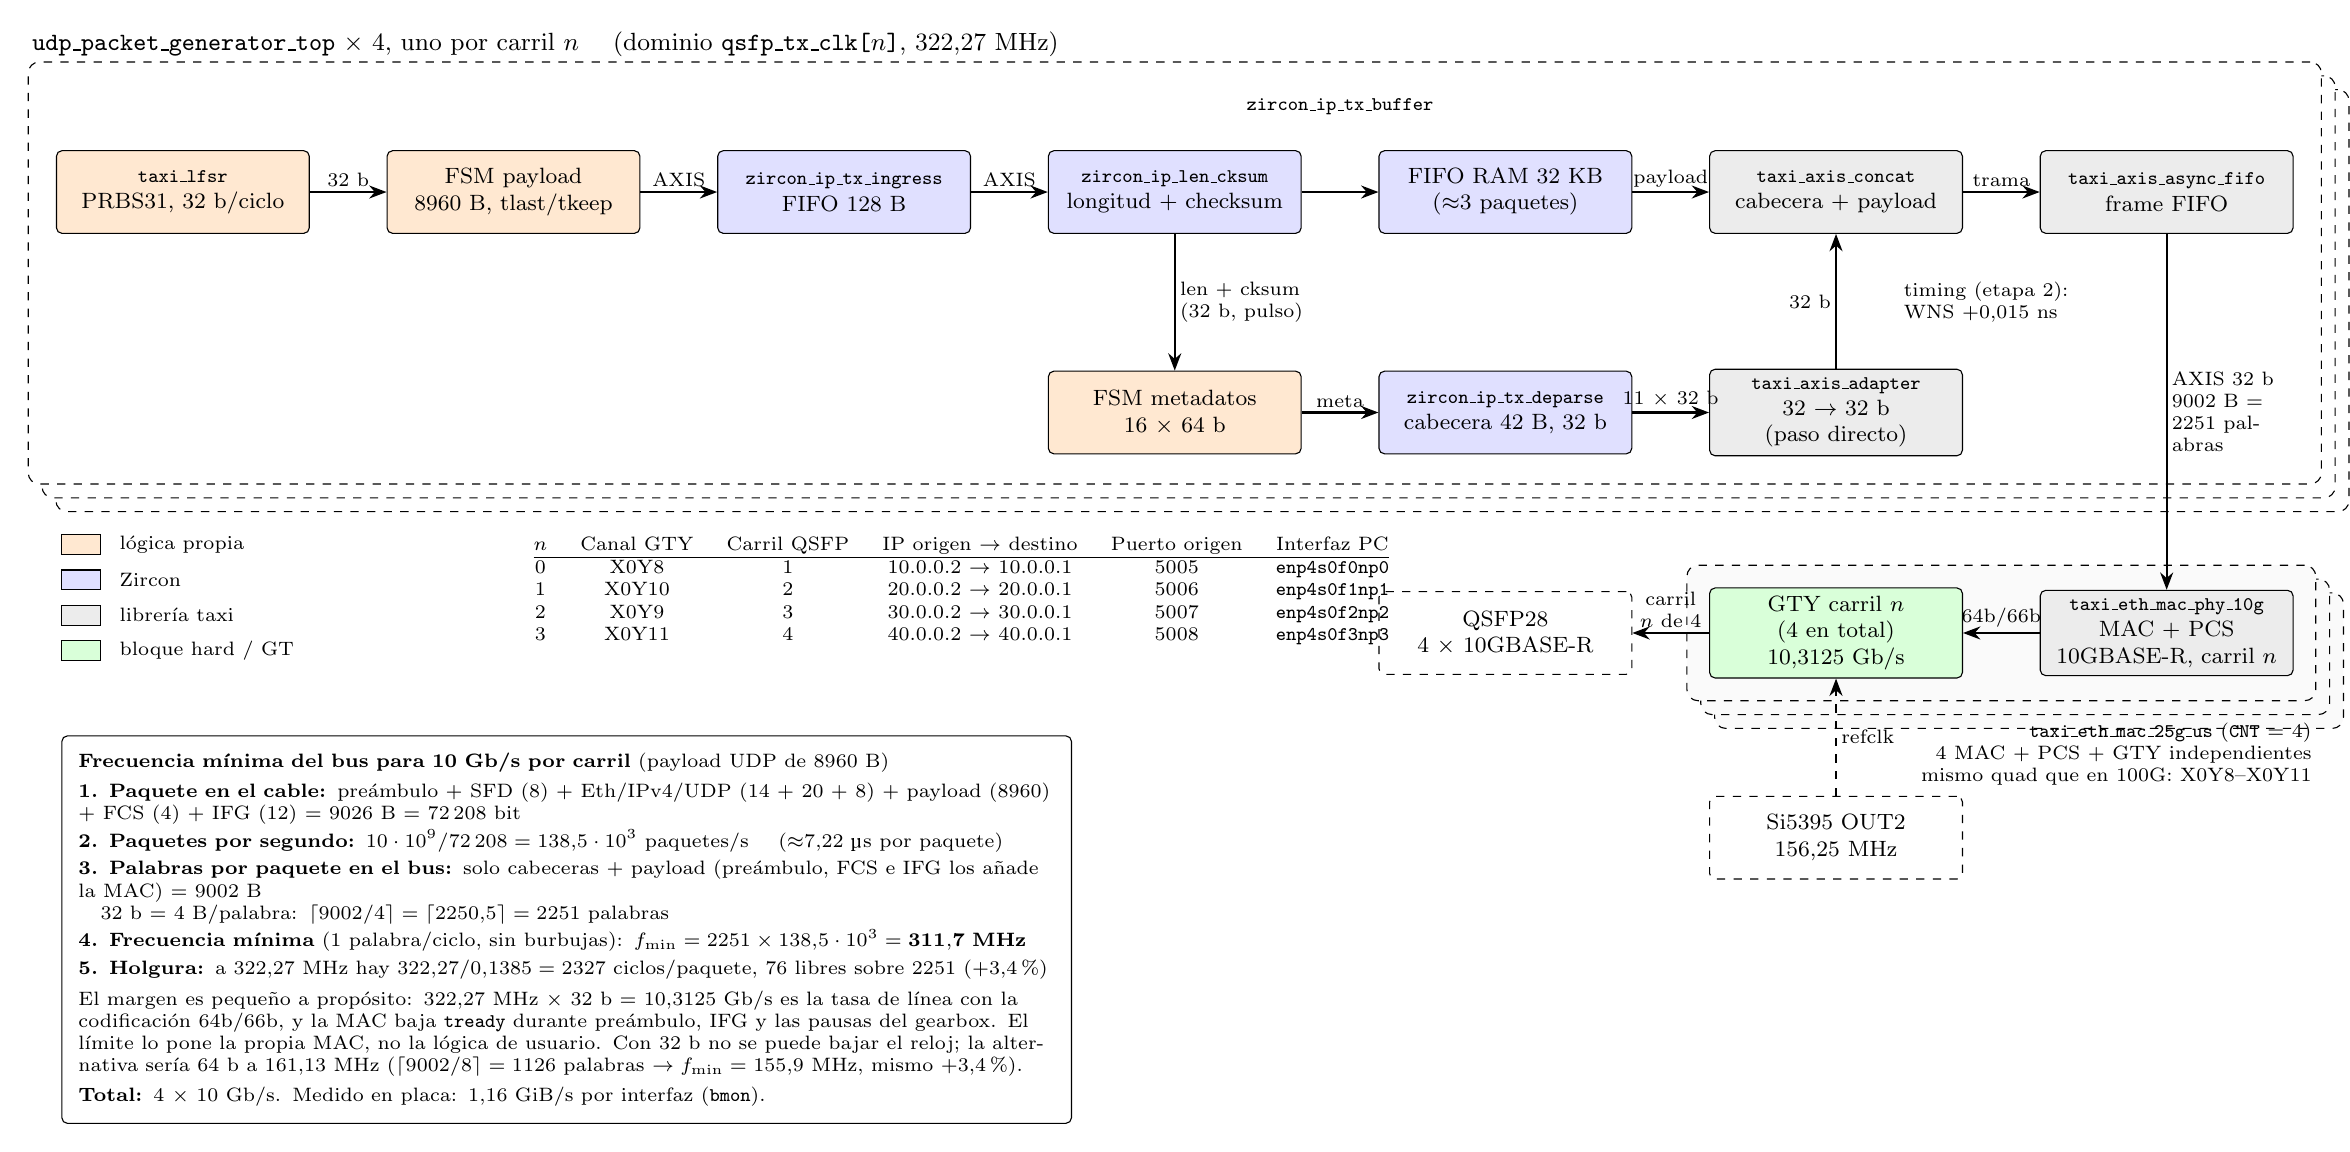
\begin{tikzpicture}[
    x=1.235cm,
    font=\footnotesize,
    >={Stealth[length=2.2mm]},
    blk/.style={draw, rounded corners=2pt, minimum height=1.05cm,
                text width=3.0cm, align=center, inner sep=3pt},
    gen/.style={blk, fill=orange!18},
    zir/.style={blk, fill=blue!12},
    taxi/.style={blk, fill=gray!15},
    soft/.style={blk, fill=gray!15},
    hard/.style={blk, fill=green!15},
    ext/.style={blk, fill=white, dashed},
    grp/.style={draw, dashed, rounded corners=4pt},
    lbl/.style={font=\scriptsize, inner sep=1.5pt},
    flow/.style={->, thick},
]

% ---------------------------------------------------------------- payload path
\node[gen]  (lfsr)    at (0,0)     {\modname{taxi\_lfsr}\\PRBS31, 32 b/ciclo};
\node[gen]  (fsmp)    at (3.4,0)   {FSM payload\\8960 B, tlast/tkeep};
\node[zir]  (ingress) at (6.8,0)   {\modname{zircon\_ip\_tx\_ingress}\\FIFO 128 B};
\node[zir]  (cksum)   at (10.2,0)  {\modname{zircon\_ip\_len\_cksum}\\longitud + checksum};
\node[zir]  (ram)     at (13.6,0)  {FIFO RAM 32 KB\\($\approx$3 paquetes)};
\node[taxi] (concat)  at (17,0)    {\modname{taxi\_axis\_concat}\\cabecera + payload};
\node[taxi] (afifo)   at (20.4,0)  {\modname{taxi\_axis\_async\_fifo}\\frame FIFO};

% ---------------------------------------------------------------- metadata path
\node[gen]  (fsmm)    at (10.2,-2.8) {FSM metadatos\\16 $\times$ 64 b};
\node[zir]  (deparse) at (13.6,-2.8) {\modname{zircon\_ip\_tx\_deparse}\\cabecera 42 B, 32 b};
\node[taxi] (adapter) at (17,-2.8)   {\modname{taxi\_axis\_adapter}\\32 $\to$ 32 b (paso directo)};

% ---------------------------------------------------------------- MAC / PHY
\node[soft] (mac)     at (20.4,-5.6) {\modname{taxi\_eth\_mac\_phy\_10g}\\MAC + PCS 10GBASE-R, carril $n$};
\node[hard] (gty)     at (17,-5.6)   {GTY carril $n$ (4 en total)\\10,3125 Gb/s};
\node[ext]  (qsfp)    at (13.6,-5.6) {QSFP28\\4 $\times$ 10GBASE-R};
\node[ext]  (si5395)  at (17,-8.2)   {Si5395 OUT2\\156,25 MHz};

% ---------------------------------------------------------------- arrows
\draw[flow] (lfsr)    -- node[lbl, above] {32 b} (fsmp);
\draw[flow] (fsmp)    -- node[lbl, above] {AXIS} (ingress);
\draw[flow] (ingress) -- node[lbl, above] {AXIS} (cksum);
\draw[flow] (cksum)   -- (ram);
\draw[flow] (ram)     -- node[lbl, above] {payload} (concat);
\draw[flow] (concat)  -- node[lbl, above] {trama} (afifo);

\draw[flow] (cksum)   -- node[lbl, right, text width=1.9cm] {len + cksum\\(32 b, pulso)} (fsmm);
\draw[flow] (fsmm)    -- node[lbl, above] {meta} (deparse);
\draw[flow] (deparse) -- node[lbl, above] {11 $\times$ 32 b} (adapter);
\draw[flow] (adapter) -- node[lbl, left] {32 b} (concat);

\draw[flow] (afifo)   -- node[lbl, right, text width=1.6cm] {AXIS 32 b\\9002 B =\\2251 palabras} (mac);
\draw[flow] (mac)     -- node[lbl, above] {64b/66b} (gty);
\draw[flow] (gty)     -- node[lbl, above, text width=1cm, align=center] {carril\\$n$ de 4} (qsfp);
\draw[flow, dashed] (si5395) -- node[lbl, right] {refclk} (gty);

% timing
\node[lbl, text width=2.6cm, align=left] at (18.75,-1.4)
    {timing (etapa 2):\\WNS +0,015 ns};

% ---------------------------------------------------------------- groups
\coordinate (gentop) at (0,1.3);
\begin{scope}[on background layer]
    \node[grp, fit=(cksum)(ram), inner xsep=6pt, inner ysep=14pt, yshift=6pt,
          fill=blue!4] (bufgrp) {};
    \node[grp, fit=(gentop)(lfsr)(afifo)(adapter), inner sep=10pt,
          fill=white, double copy shadow={shadow xshift=5pt, shadow yshift=-5pt}] (gengrp) {};
    \node[grp, fit=(gty)(mac), inner sep=8pt, fill=gray!4,
          double copy shadow={shadow xshift=5pt, shadow yshift=-5pt}] (macgrp) {};
\end{scope}
\node[lbl, anchor=north] at (bufgrp.north) {\texttt{zircon\_ip\_tx\_buffer}};
\node[lbl, anchor=south west, font=\small] at (gengrp.north west)
    {\texttt{udp\_packet\_generator\_top} $\times$ 4, uno por carril $n$
     \quad (dominio \texttt{qsfp\_tx\_clk[$n$]}, 322,27 MHz)};
\node[lbl, anchor=north east, align=right] at ([yshift=-6pt]macgrp.south east)
    {\texttt{taxi\_eth\_mac\_25g\_us} (\texttt{CNT} = 4)\\4 MAC + PCS + GTY independientes\\mismo quad que en 100G: X0Y8--X0Y11};

% ---------------------------------------------------------------- legend
\begin{scope}[shift={(-1.25,-4.6)}, every node/.style={font=\scriptsize, anchor=west}]
    \draw[fill=orange!18] (0,0)     rectangle +(0.4,0.25); \node at (0.5,0.125)  {lógica propia};
    \draw[fill=blue!12]   (0,-0.45) rectangle +(0.4,0.25); \node at (0.5,-0.325) {Zircon};
    \draw[fill=gray!15]   (0,-0.9)  rectangle +(0.4,0.25); \node at (0.5,-0.775) {librería taxi};
    \draw[fill=green!15]  (0,-1.35) rectangle +(0.4,0.25); \node at (0.5,-1.225) {bloque hard / GT};
\end{scope}

% ---------------------------------------------------------------- lane table
\node[anchor=north west, font=\scriptsize, inner sep=0pt] at (3.6,-4.35) {%
    \begin{tabular}{@{}cccccc@{}}
        $n$ & Canal GTY & Carril QSFP & IP origen $\to$ destino & Puerto origen & Interfaz PC\\\hline
        0 & X0Y8  & 1 & 10.0.0.2 $\to$ 10.0.0.1 & 5005 & \texttt{enp4s0f0np0}\\
        1 & X0Y10 & 2 & 20.0.0.2 $\to$ 20.0.0.1 & 5006 & \texttt{enp4s0f1np1}\\
        2 & X0Y9  & 3 & 30.0.0.2 $\to$ 30.0.0.1 & 5007 & \texttt{enp4s0f2np2}\\
        3 & X0Y11 & 4 & 40.0.0.2 $\to$ 40.0.0.1 & 5008 & \texttt{enp4s0f3np3}\\
    \end{tabular}};

% ---------------------------------------------------------------- budget
\node[draw, rounded corners=2pt, anchor=north west, text width=12.4cm, align=left,
      font=\scriptsize, inner sep=6pt] at (-1.25,-6.9) {%
    \textbf{Frecuencia mínima del bus para 10 Gb/s por carril} (payload UDP de 8960 B)\\[3pt]
    \textbf{1. Paquete en el cable:}
    preámbulo + SFD (8) + Eth/IPv4/UDP (14 + 20 + 8) + payload (8960) + FCS (4) + IFG (12)
    = 9026 B = 72\,208 bit\\[2pt]
    \textbf{2. Paquetes por segundo:}
    $10\cdot10^{9} / 72\,208 = 138{,}5\cdot10^{3}$ paquetes/s
    \quad($\approx$7,22 µs por paquete)\\[2pt]
    \textbf{3. Palabras por paquete en el bus:}
    solo cabeceras + payload (preámbulo, FCS e IFG los añade la MAC) = 9002 B\\
    \hspace*{1em}32 b = 4 B/palabra: $\lceil 9002/4 \rceil = \lceil 2250{,}5 \rceil = 2251$ palabras\\[2pt]
    \textbf{4. Frecuencia mínima} (1 palabra/ciclo, sin burbujas):
    $f_{\min} = 2251 \times 138{,}5\cdot10^{3} = \mathbf{311{,}7\ MHz}$\\[2pt]
    \textbf{5. Holgura:} a 322,27 MHz hay $322{,}27 / 0{,}1385 = 2327$ ciclos/paquete,
    76 libres sobre 2251 (+3,4\,\%)\\[3pt]
    El margen es pequeño a propósito: 322,27 MHz $\times$ 32 b = 10,3125 Gb/s es la tasa de línea
    con la codificación 64b/66b, y la MAC baja \texttt{tready} durante preámbulo, IFG y las pausas
    del gearbox. El límite lo pone la propia MAC, no la lógica de usuario. Con 32 b no se puede
    bajar el reloj; la alternativa sería 64 b a 161,13 MHz
    ($\lceil 9002/8 \rceil = 1126$ palabras $\to f_{\min} = 155{,}9$ MHz, mismo +3,4\,\%).\\[3pt]
    \textbf{Total:} 4 $\times$ 10 Gb/s. Medido en placa: 1,16 GiB/s por interfaz (\texttt{bmon}).};

\end{tikzpicture}
\end{document}
